\section{Teilbericht Simulation}
Der Teilbericht der Simulationsgruppe beschreibt die entwickelte Simulationssoftware von der Anforderungsanalyse über die Implementierung hin zum Testen und Validieren. 
\subsection{Lastenheft}
Mit der Komponente Simulation soll auf Basis des Ablaufkonzepts eine Software erstellt werden, die es erlaubt, einen automatisierten Materialfluss auf Basis von FTS zu simulieren, ohne dabei an die zahlenmäßigen Beschränkungen des physischen Systems gebunden zu sein. Vonseiten des Auftraggebers wurde ein Lastenheft vorgegeben, das die gewünschten Kernfunktionalitäten der Simulationssoftware beschreibt. Es enthält folgende Anforderungen:
\begin{enumerate}
\item \textbf{Akteure}: Die virtuellen Akteure sind in ihrem Verhalten und Eigenschaften (Geschwindigkeit, Dauer einer Paketübergabe etc.) den echten Objekten aus dem physischen System nachempfunden (Volksbots und passive Rampen).
\item \textbf{Ablauf}: Der in Abschnitt 4.1 beschriebene Ablauf wird in der Simulation umgesetzt. 
\item \textbf{Visualisierung}: Die Zustände der Akteure werden dynamisch visualisiert. Wird beispielsweise die Anzahl der Pakete auf einer Rampe um eins erhöht, dann soll dies unmittelbar in der Anzeige visualisiert werden.
\item \textbf{Generierung von Aufträgen}: Eingehende und ausgehende Transportaufträge können erstellt und simuliert werden. 
\item \textbf{Einstellungen}: Verschiedene Parameter der Simulation (Anzahl und Art der Akteure, Anzahl der Aufträge etc.) können vom Nutzer vor dem Starten der Simulation angepasst werden.
\item \textbf{Statistiken}: Es werden wichtige Daten geloggt, um am Ende eines Simulationslaufs aussagekräftige Analysen über Stromverbrauch, gefahrene Strecken, Vergabe von Aufträgen usw. machen zu können.
\end{enumerate}
\subsection{Grundlegende Designentscheidungen}
Vor der Entwicklung der Simulationssoftware mussten grundlegende Designentscheidung getroffen werden. Zum einen musste entschieden werden, ob die Simulation von einem autonomen Lager auf Basis eines vorhanden Tools oder komplett neu entwickelt werden sollte. Auch musste zwischen Desktop- und Webanwendung entschieden werden und ob die jeweilige Alternative mit oder ohne Zuhilfenahme eines Frameworks implementiert wird. In den nachfolgenden Abschnitten werden die getroffenen Designentscheidungen begründet.
\subsubsection{Eigenentwicklung}
Im Vorfeld der Entwicklung wurde der Teilgruppe Simulation das Player/Stage Tool als Alternative zu einer kompletten Neuentwicklung einer Software vorgeschlagen. Das Tool beinhaltet zum einen die Komponente Player, die eine Hardware Abstraktionsschicht darstellt. Mit dieser Komponente kann mit Robotern, wie beispielsweise einem Volksbot, interagiert werden, ohne dass technische Details der Komponenten (Laserscanner, Motor etc.) bekannt sein müssen. Auf Basis von selbstgeschriebenem Code können Roboter gesteuert werden. Die Komponente Stage horcht auf die Befehle, die Player ausführt und visualisiert diese in einem eigenen Graphical User Interface. Jedoch kann Stage auch ohne Hardware benutzt werden, indem man über Konfigurationsdateien ein eigenes Szenario erstellt und die virtuellen Roboter über den eigenen Code steuert. Somit bietet das Tool die Möglichkeit, eine Simulation mit Robotern zu erstellen und das gewünschte Verhalten der Roboter über eigenen Code abzubilden. Auch muss die Visualisierung nicht selbst entwickelt werden (Vgl.\cite{plstg}). 
\\\\
Dennoch wurde eine Eigenentwicklung der Nutzung des Tools vorgezogen. Die Benutzeroberfläche von Stage bietet die Möglichkeit, die Anzahl der Roboter und das Layout eines Szenarios über die entsprechenden Konfigurationsdateien einzustellen (Vgl.\cite{plstg}). Jedoch gibt es beispielsweise keine Möglichkeit Aufträge zu erstellen bzw. zu simulieren oder Statistiken anzuzeigen. Somit ist die Entwicklung einer eigenen Benutzeroberfläche unumgänglich. Das bedeutet, dass die Stage Oberfläche über eine eigene Benutzeroberfläche gesteuert werden muss. Somit hätte man eine Trennung zwischen Visualisierung und Konfiguration eines Szenarios, was die Benutzerfreundlichkeit erheblich beeinträchtigt, da ein Nutzer den Durchlauf einer Simulation über zwei Benutzeroberflächen hinweg verfolgen müsste. Die Entwicklung eines eigenen Systems bietet somit erheblich mehr Benutzerfreundlichkeit und ermöglicht es, alle Anforderungen an das Interface in einer Benutzeroberfläche zu integrieren. 
\subsubsection{Entwicklung einer Webanwendung}\label{sec:Entwicklung einer Webanwendung} 
Die Software soll als Webanwendung implementiert werden. Gegenüber einer Desktopanwendung bietet eine Webapplikation folgende Vorteile:
\begin{itemize}
\item Das System ist plattformunabhängig und kann somit auf jedem Rechner, der über einen Webbrowser verfügt, ausgeführt werden.
\item Die Software muss nicht lokal installiert werden und kann direkt genutzt werden.
\item Werden Änderungen an der Software vorgenommen, sind diese direkt verfügbar, da Updates über den Webserver eingespeist werden. Die Software ist somit immer auf dem aktuellsten Stand. 
\end{itemize}
\subsubsection{Umsetzung durch GWT}\label{GWT} 
Die Entwicklung der Webanwendung sollte mithilfe eines Frameworks erfolgen, das es erlaubt, den Code sowohl für die Client- als auch für die Serverseite in einer Programmiersprache zu entwickeln. Außerdem sollte das Framework Schnittstellen bieten, um asynchrone Kommunikation und Push-Dienste zu nutzen, ohne sich um die exakten Details kümmern zu müssen. Ausgewählt wurde das Google Web Toolkit (GWT). GWT ist ein von Google entwickeltes Framework zur Erstellung von Webanwendungen. Der Java-Code für den Client wird von dem GWT Compiler in den entsprechenden Javascript- und HTML-Code übersetzt. Somit kann die Entwicklung sowohl für Client als auch für den Server auf Basis von Java erfolgen. Zudem entfällt die Anpassung des Javascript-Codes für die verschiedenen Browser, da GWT beim Kompilieren automatisch für jeden Browser eine lauffähige Version erzeugt. Weiterhin besitzt GWT  eine RCP-Schnittstelle für die asynchrone Kommunikation zwischen Client und Server und lässt sich um Komponenten erweitern, um Daten vom Server zum Client zu pushen (Vgl.\cite{gwt}). Somit erfüllt GWT sämtliche an ein Framework gestellte Anforderungen. Weitere Alternativen wurden nicht in Betracht gezogen, da drei von fünf Mitgliedern der Teilgruppe Simulation bereits positive Erfahrungen mit GWT gemacht haben und die anderen Mitglieder somit schnell einarbeiten konnten. 
\subsection{Konzeption der Systemkomponenten}
In diesem Abschnitt wird die Konzeption der Gesamtarchitektur als auch der einzelnen Systemkomponenten beschrieben, die im Rahmen der Sprints erarbeitet wurde. Die Konzeption beinhaltet zum einen die Anforderungen, als auch die daraus abgeleiteten Implementierungsvorgaben.
\newpage
\subsubsection{Gesamtarchitektur}\label{GA} 
Wie in Kapitel \ref{sec:Entwicklung einer Webanwendung} beschrieben, soll die Software als Webanwendung realisiert werden. Eine Webanwendung erfordert eine Client-Server Architektur. Abbildung \ref{Gesamtarchitektur} beschreibt die wesentlichen Komponenten des Systems und wie diese sich auf die Client- und Serverseite verteilen. Basis der Anwendung ist der Webserver, der die Basiskomponenten des Systems hosted. Zum einen stellt er die Laufzeitumgebung für Webanwendung und Datenbank bereit. Die Datenbank wird benötigt, um Daten, wie beispielsweise erstellte Szenarien, persistent zu speichern. Aus der Webanwendung heraus kann auf die Datenbank lesend und schreibend zugegriffen werden. In die Webanwendung soll ein Multiagentensystem (MAS) eingebettet werden. Ein MAS ist ein Netzwerk aus Softwareagenten. Softwareagenten sind Softwareeinheiten, die in in der Lage sind, Aufgaben selbstständig durchzuführen (Vgl.\cite{mas}). Mithilfe des MAS kann ein Lager simuliert werden, in dem der Warenfluss durch vollständig autonome Akteure durchgeführt wird. 
\\\\
Der Webserver beinhaltet die Logik des Systems. Auf dem Client soll die Visualisierung erfolgen und der Nutzer soll das Starten einer Simulation initiieren können. Das System soll von einem Webbrowser aus aufrufbar sein, in dem die Ergebnisse der serverseitigen Prozesse dargestellt werden. Mehrere Nutzer sollen das System gleichzeitig nutzen können, ohne Login und Registrierung.

\begin{figure}[h!]
	\centering
		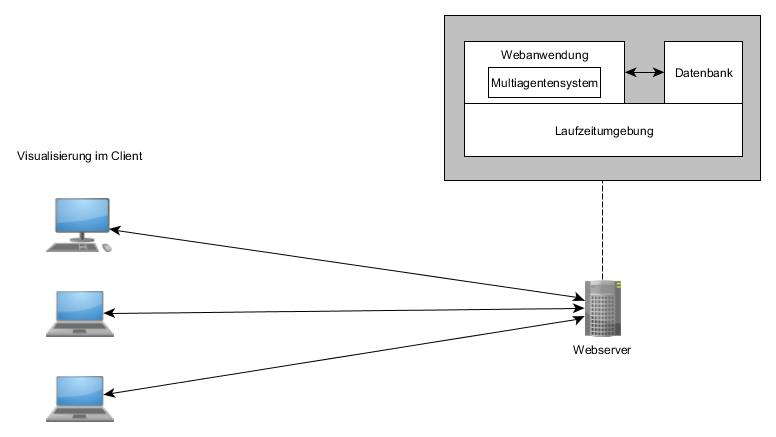
\includegraphics[width=0.8\textwidth]{grobarchitektur.jpg}        
		\caption{Gesamtarchitektur}
	\label{Gesamtarchitektur}
\end{figure} 
\newpage
\subsubsection{Konzeption der Benutzeroberfläche}
Die Benutzeroberfläche soll einem Nutzer die Möglichkeit bieten, auf sämtliche Funktionalitäten, die für die Durchführung eines Simulationsdurchlaufs relevant sind, zuzugreifen. Abbildung \ref{GUI} zeigt den schematischen Aufbau der Gui anhand eines Mockups. Die Menüleiste beinhaltet drei Menu Items: Simulation, Auftragsliste und Statistiken. Über die Items Simulation und Auftragsliste sollen erstellte Szenarien und Auftragslisten geladen und gespeichert werden können. Außerdem soll eine Simulation gestartet werden können. Das Statistik Item erlaubt den Zugriff auf Statistiken, die für einen Durchlauf generiert wurden. Links unter der Menüleiste befindet sich die Auftragsliste, über die Aufträge generiert und angezeigt werden können. Darunter befindet sich der Bereich, der für die Modellierung eines Szenarios relevant ist. Es sollen Rampen, Fahrzeuge und Wände als Modellelemente auswählbar sein und in der Zeichenfläche platziert werden können. Die Zeichenfläche selber befindet sich rechts unter der Menüleiste. Dort werden die Aktionen der Akteure, wie z.~B. Aufladen eines Pakets, visualisiert. Das unterste Element enthält eine Debug-Konsole, in der serverseitige Aktionen dargestellt werden können, die nicht in der Zeichenfläche dargestellt werden sollen. 
\begin{figure}[h!]
	\centering
		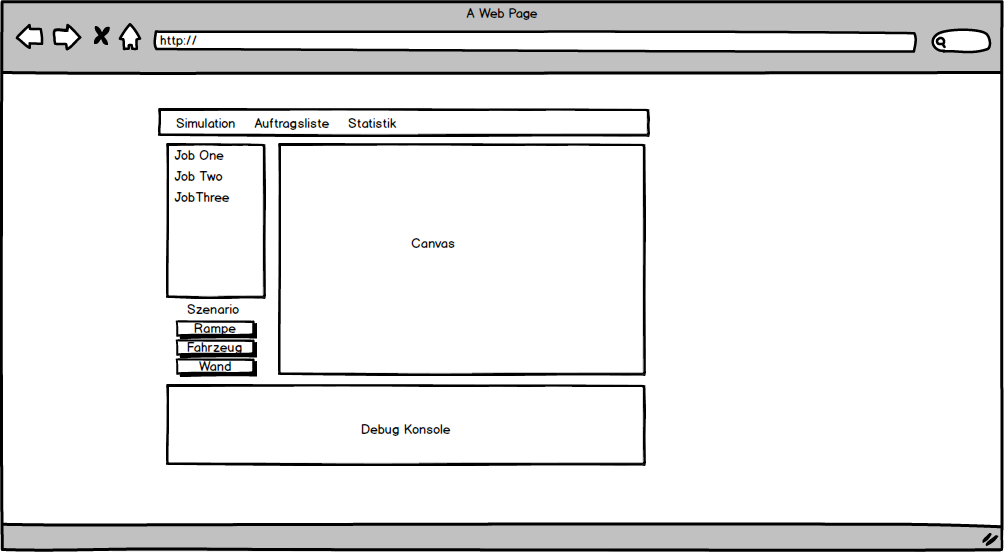
\includegraphics[width=0.8\textwidth]{Mockup.png}        
		\caption{Schematischer Aufbau der Benutzeroberfläche}
	\label{GUI}
\end{figure}
\subsubsection{Generierung von Aufträgen}
Die Simulationssoftware soll ein Umschlagslager simulieren. Das bedeutet, dass Pakete in das Lager geliefert, zwischengelagert und an den Ausgangsrampen wieder abgeholt werden, wenn ein bestimmtes Paket angefragt wird (Vgl.\ref{Einsatzszenario}). Das bedeutet, dass eine Unterscheidung getroffen werden muss zwischen einem physischen Paket und einer Nachfrage nach einem bestimmten Paket, die ein Ausgang stellt. Deshalb soll zwischen eingehenden und ausgehenden Aufträgen unterschieden werden. Es soll möglich sein, eine festgelegte Anzahl an Aufträgen zufällig über die Gui zu generieren. Außerdem muss sichergestellt werden, dass die Menge an generierten eingehenden und ausgehenden Aufträgen in einem bestimmten Verhältnis zueinander stehen, um zu verhindern, dass nur eingehende oder nur ausgehende Aufträge generiert werden. 
\subsubsection{Anforderungen an ein Multiagenten-Framework}
Um ein Umschlagslager und die darin enthaltenden Akteure (Rampen und Fahrzeuge) zu simulieren, wird ein Multiagentensystem benötigt (Vgl.\ref{GA}). Zur Erstellung eines MAS soll ein Framework verwendet werden, dass die nachfolgenden Anforderungen erfüllt: Das Framework muss das Erstellen von verschiedenen Agententypen ermöglichen, um die Akteure und ihre spezifischen Aufgabenstellungen umzusetzen. Agenten müssen in der Lage sein, untereinander Nachrichten auszutauschen und auf bestimmte Nachrichten oder Ereignisse mit definierten Verhaltensweisen zu reagieren. Weiterhin sollen die Aktionen der Agenten denen der realen Akteure hinsichtlich der Dauer ähneln. Außerdem muss das Framework Aktionen von verschiedenen Agenten parallel ausführen können, damit beispielsweise das gleichzeitige Fahren mehrerer Fahrzeuge möglich ist.
\subsubsection{Benötigte Agententypen}
Sowohl Rampen als auch Fahrzeuge müssen verschiedene Aktionen durchführen. Dazu gehören u.~a. das Befördern von Paketen, die Vergabe von Aufträge, Durchführung von Auktionen usw. Würde man alle Aufgaben, die ein Akteur durchführen muss, in einem Agenten bündeln, so wäre ein solcher Agent nur schwer wartbar und es könnten abhängig vom Agenten-Framework Probleme bei der Parallelisierung von Aktionen auftreten. Es bietet sich an, die erforderlichen Aufgaben eines Akteurs auf mehreren Agenten zu verteilen. Durch die Modularisierung kann die Entwicklung des Systems parallelisiert werden und Änderungen an einem Agenten haben geringere Auswirkungen auf das Gesamtsystem. Die Wartbarkeit des Systems erhöht sich. Für das zu entwickelnde System wurden die folgenden vier Agententypen konzipiert:  
\begin{itemize}
\item Paketagent: Verwaltung der Paketdaten
\item Orderagent: Ermittlung von Zielrampen und Zuweisung von Zielen (Wird nur bei Rampen benötigt)
\item Routingagent: Durchführung von Auktionen und Berechnung von möglichen Pfaden
\item Plattformagent: Durchführung physischer Aktionen (Fahren, Aufladen von Paketen etc.)
\end{itemize}
\subsubsection{Kommunikation zwischen den Agenten}
Die zu entwickelnde Software soll die in Abschnitt \ref{AL} beschriebenen Abläufe umsetzen. Die Aufgaben der verschiedenen Akteure müssen auf die Agenten verteilt werden. Die entworfenen Kommunikationsschritte der Agenten sollen für den Fall dass ein Eingang Ausgänge und Zwischenlager fragt, beschrieben werden, um die Aufgaben der einzelnen Agenten genauer abzugrenzen. Im Rahmen der Implementierung können sich noch Änderungen ergeben, die technisch notwendig sind. 
\begin{enumerate}
\item Trifft ein Paket ein, verlangt der Paketagent vom Orderagenten eine Destination für das entsprechende Paket.
\item Der Orderagent einer Eingangsrampe fragt die Orderagenten der Ausgangs- und Zwischenrampen.
\item Die Orderagenten prüfen im Abgleich mit ihren Paketagenten, ob Platz frei ist (Zwischenrampe) oder die Paket-ID benötigt wird (Ausgang). Anschließend antworten sie dem Orderagenten am Eingang.  
\item Wurde ein Ziel für das Paket gefunden, soll der Orderagent den Start einer Auktion initiieren, indem er den Routingagenten benachrichtigt. 
\item Der Routingagent verlangt eine Aufwandsschätzung von allen Routingagenten der Fahrzeuge.
\item Der Routingagent eines Fahrzeugs berechnet eine Aufwandsschätzung anhand seiner Position und antwortet dem Routingagenten der Rampe. Fährt der Volksbot oder nimmt er an einer anderen Auktion teil, so wird -1 als Aufwandsschätzung zurückgeschickt.
\item Der Routingagent einer Rampe wählt, sofern vorhanden, den Bot aus, der den geringsten Aufwand benötigt, um ein Paket abzuholen und weist ihm den Auftrag zu.
\item Der Plattformagent fährt zu der jeweiligen Eingangsrampe und lädt das Paket auf. Dies geschieht durch einen Nachrichtenaustausch mit dem jeweiligen Plattformagenten der Rampe, der die Paketdaten übergibt. Das Fahren zur Zielrampe und das Abladen des Pakets erfolgt analog. 
\end{enumerate}
\subsubsection{Konzeption des Pathfindings}
\subsubsection{Konzeption der Statistiken}
\subsubsection{Interaktion der Komponenten} \label{Interaktion der Komponenten}
Durch das Zusammenspiel der Komponenten der verschiedenen Systemkomponenten soll eine Simulation durchgeführt werden können. Die Aufträge müssen entsprechend ihrer Zeiten an den Server geschickt werden. Dies soll clientseitig durch einen Timer durchgeführt werden, um das MAS zu entlasten. Abbildung \ref{Int} zeigt den Ablauf und die Komponenten, die für das Starten einer Simulation erforderlich sind: 
\begin{enumerate}
\item Ein potenzieller Nutzer startet eine Simulation über die Benutzeroberfläche.
\item Der Server wird durch die GUI informiert, dass die Simulation gestartet werden soll.
\item Der Server startet das Multiagentensystem.
\item Der Server meldet dem Client den Start des MAS.
\item Der Client weiß nun, dass die Agenten bereit sind, Aufträge entgegenzunehmen und startet den Timer für die Jobliste.
\item Die Aufträge werden gemäß ihrer Startzeit an den Server geschickt.
\item Der Server leitet die Aufträge an das MAS weiter
\item Die Daten über sichtbare Zustandsveränderungen werden an den Client geschickt und dort in der GUI visualisiert.
\end{enumerate}

\begin{figure}[h!]
	\centering
		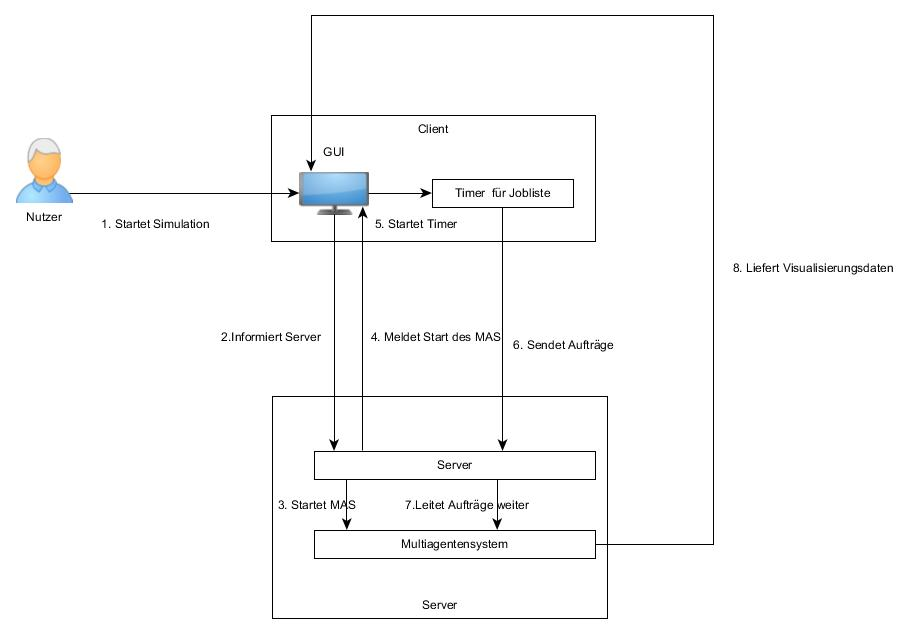
\includegraphics[width=0.8\textwidth]{Interaktion.jpg}        
		\caption{Interaktion der Systemkomponenten}
	\label{Int}
\end{figure}
\newpage
\subsection{Implementierung der Systemkomponenten}
In diesem Abschnitt soll die Implementierung der zuvor konzipierten Systemkomponenten beschrieben werden. Zum einen soll die Auswahl von Technologien und Frameworks zur Umsetzung beschrieben sowie die Funktionalität des Systems auf technischer Ebene dargestellt werden.
\subsubsection{Implementierte Gesamtarchitektur}
Abbildung \ref{GAI} zeigt die konkrete Gesamtarchitektur des Systems, die durch die Auswahl von Umsetzungstechnologien entstanden ist. Die Webanwendung soll, wie bereits in Abschnitt \ref{GWT} beschrieben, durch das GWT Framework implementiert werden. Der Code für Server und Client, der für Visualisierung, Client-Server Kommunikation u.~ä., benötigt wird, wird durch GWT-Bilbiotheken bereitgestellt. Eingebettet in die GWT-Klassen wird das Multiagentensystem, das mithilfe des Java Agent Development Framework (JADE)\footnote{\cite{jade}} implementiert wurde. Als Datenbankmanagementsystem wurde PostgreSQL ausgewählt. Die Applikation wird durch einen Jetty Server gehostet, der die Java Laufzeitumgebung und das GWT Software Development Kit ebenfalls bereitstellt.  
\begin{figure}[h!]
	\centering
		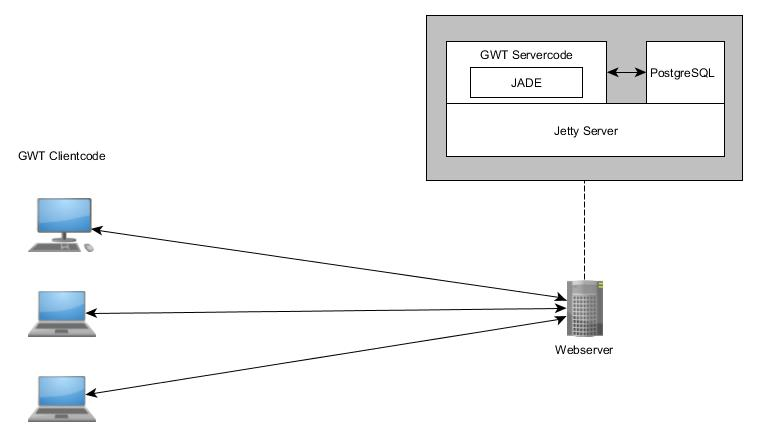
\includegraphics[width=0.8\textwidth]{architekturSimu.jpg}        
		\caption{Implementierte Gesamtarchitektur}
	\label{GAI}
\end{figure}
\subsubsection{Benutzeroberfläche}
\subsubsection{Generierung von Aufträgen}
\subsubsection{Auswahl eines Multiagenten-Frameworks}
Das Java Agent Development Framework wurde genutzt, um ein Netzwerk aus verschiedenen Agenten zu implementieren. Jade erlaubt das Erstellen von verschiedenen Agenten. Agenten werden als Java-Klasse implementiert, die von der vordefinierten Klasse Agent erbt. Die Aktionen, die ein Agent ausführen soll, werden durch Behaviours implementiert, die ebenfalls Klassen sind. Um die Anzahl an Klassen zu reduzieren, wurden die Behaviours als interne Klassen in die Agenten eingefügt. Jade ermöglicht die Kommunikation zwischen den Agenten durch ein vordefiniertes Nachrichtensystem. Nachrichten können sowohl gezielt an einen Agenten adressiert oder an alle Agenten verschickt werden. Die Agenten können in Echtzeit miteinander kommunizieren und mehrere Agenten können parallel Aktionen ausführen, da jeder Agent in einem eigenen Thread läuft (Vgl.\cite{jadetwo}). 
\subsubsection{Implementierte Agententypen}
Implementiert wurden sieben verschiedene Agententypen. Jede Rampe besitzt jeweils einen Paket-, Order-, Routing- und Plattformagenten. Ein Fahrzeug besitzt einen Paket-, Routing- und Plattformagenten. Die Routing- und Plattformagenten wurden für Fahrzeuge und Rampen durch unterschiedliche Agenten implementiert, um die Anzahl an Behaviours pro Agent zu reduzieren und den Code übersichtlicher zu gestalten und unnötigen Speicherverbrauch zu vermeiden. Damit ein Agent weiß, welchem Szenario und welchem Akteur er zugeordnet ist, werden Szenario und Conveyor als Referenz übergeben \footnote{Der genaue Ablauf der Initialisierung wird in Abschnitt \ref{Interaktion der Komponenten} beschrieben}. Neben den genannten Agenten war es notwendig, einen Jobagent zu implementieren, der die Übergabe eines Pakets, die im phyischen System durch einen Menschen geschieht, zu simulieren. Außerdem werden ausgehende Aufträge durch den Jobagent an die Ausgangsrampen übermittelt.
\subsubsection{Kommunikation zwischen den Agenten}
In den nachfolgenden Abschnitten soll die Kommunikation zwischen den Agenten, die implementiert wurde, anhand von Sequenzdiagrammen beschrieben werden. Dabei werden folgende Anwendungsszenarien durchlaufen:
\begin{itemize}
\item Jobzuweisung an Ein- und Ausgänge.
\end{itemize}

\paragraph{Jobzuweisung an Ein- und Ausgänge} \label{Jobagent}
Abbildung \ref{Job} zeigt die Jobzuweisung an die Ein- und Ausgangsrampen durch den Jobagent. Bevor die Jobzuweisung beginnt, wird die Simulation durch den Client gestartet. Neben dem Jobagent, den Plattformagenten der Rampen und dem Paketagenten ist das Servlet AgentPlattformServiceImpl an der Kommunikation beteiligt. Auf die Aspekte der Client-Server Kommunikation wird in Abschnitt  \ref{Interaktion der Komponenten} genauer eingegangen. Das Diagramm zeigt folgenden Ablauf:
\begin{itemize}
\item Die Simulation wird aus dem Browser heraus gestartet und das Servlet wird benachrichtigt.
\item Das Servlet startet die Agentenplattform und initialisiert die Agenten, einschließlich dem Jobagent. 
\item Der Jobagent startet einmalig eine Anfrage an die Plattformagenten der Rampen, um die IDs und die Anzahl der Ein- und Ausgänge zu erfragen, die für die Jobzuweisung nötig sind. 
\item Die Plattformagenten senden ihren Rampentyp an den Jobagent.
\item Der Jobagent besitzt zwei Listen in denen er die IDs, der Ein- und Ausgänge speichert. Anhand des empfangenen Rampentyps, speichert er die ID des Senders in der entsprechenden Liste. Anschließend wird der Client benachrichtigt, dass die Simulation gestartet wurde.
\item Der Client startet den Jobtimer und sendet die Aufträge entsprechend ihrer zeitlichen Reihenfolge an das Servlet.
\item Das Servlet leitet die Aufträge an den Jobagent weiter.
\item Der Jobagent empfängt den Auftrag und sendet eine Nachricht an sich selbst.
\item Je nach Art des Auftrags werden entweder die Eingangs- oder Ausgangsrampen gefragt, ob der Auftrag entgegengenommen werden kann.
\item Die Plattformagenten senden eine Nachricht an ihre Paketagenten, um zu prüfen, ob der Auftrag aufgenommen werden kann. Der Plattformagent wartet auf die Antwort des Paketagenten.
\item Der Paketagent prüft, ob der Auftrag entgegengenommen werden kann und antwortet dem Plattformagent.
\item Der Plattformagent verarbeitet die Anfrage und antwortet dem Jobagent. Läuft der Plattformagent auf einer Ausgangsrampe, so wird automatisch geantwortet, dass Platz verfügbar ist, da ausgehende Aufträge nur IDs repräsentieren, die der Ausgang anfragt. Ein Ausgang kann unbegrenzt IDs anfragen.
\item Der Jobagent wählt unter den Rampen, die einen Auftrag entgegennehmen können, zufällig eine aus und sendet die Auftragsdaten an den Plattformagenten.
\item Der Plattformagent initialisiert mit den Auftragsdaten die Paketdaten und schickt diese an den Paketagenten. Zu beachten ist, dass die Klasse PackageDate sowohl eingehende als auch ausgehende Aufträge repräsentiert.
\item Der Paketagent fügt das Paket einer Liste hinzu.
\end{itemize}   
\begin{figure}[h!]
	\centering
		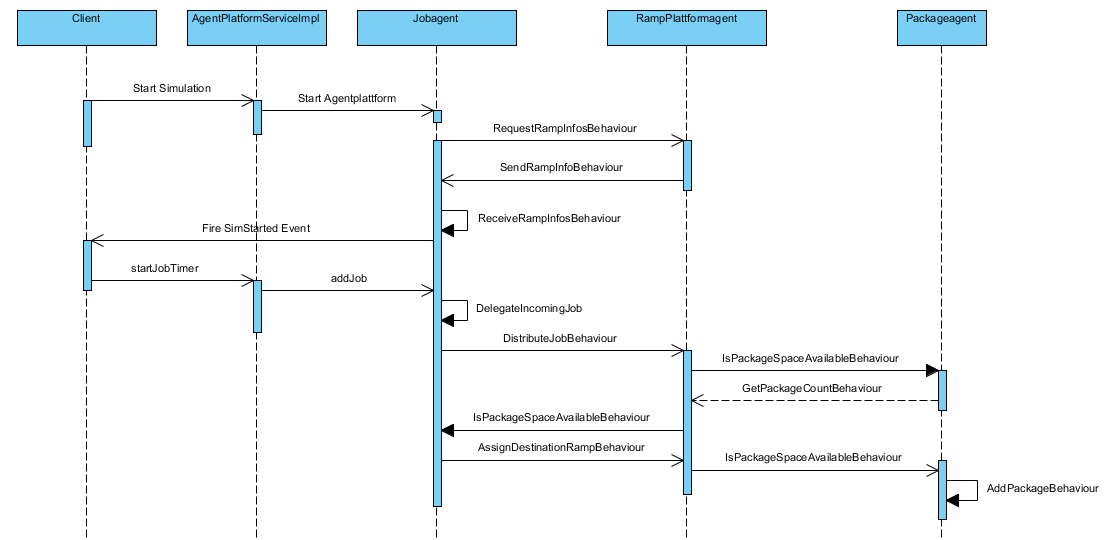
\includegraphics[width=1.1\textwidth, height=0.6\textwidth]{Jobagent.png}        
		\caption{Jobzuweisung an Ein- und Ausgänge}
	\label{Job}
\end{figure}
\newpage
\paragraph{Eingang fragt Ausgang und Zwischenlager}
Pakete, die am Eingang eintreffen, werden weitergeleitet. Besteht ein Bedarf am Ausgang, so soll das Paket zum Ausgang befördert werden. Ansonsten wird es ins Zwischenlager gebracht. Abbildung \ref{Eingang fragt} zeigt den Nachrichtenaustausch der Agenten, der zur Zielfindung nötig ist:
\begin{itemize}
\item Der Paketagent stellt mithilfe einer Tickerbehaviour zyklisch Anfragen an seinen Orderagenten, um ein Ziel für das vorderste Paket zu bekommen. Bevor der Orderagent benachrichtigt wird, prüft der Paketagent mithilfe der Variable OutgoingJobFlag, ob für das Paket bereits ein Ziel gefunden wurde. Falls nicht, sendet er die Anfrage an den Orderagenten.  
\item Der Orderagent sendet eine Nachricht an alle Orderagenten der Ausgangs- und Zwischenrampen.
\item Der jeweilige Orderagent fragt seinen Paketagenten, ob bereits ein Paket erwartet wird. Dies ist nötig, damit sich nicht mehrere Bots vor einer Rampe blockieren.
\item Der Paketagent prüft anhand der Variable IncomingJobFlag, ob ein Paket erwartet wird und antwortet seinem Orderagenten.
\item Sofern kein Paket erwartet wird, fährt der Orderagent fort und stellt eine erneute Anfrage an seinen Paketagenten, um zu fragen, ob das entsprechende Paket benötigt wird (Ausgang) oder ob Platz frei ist (Zwischenlager).
\item Der jeweilige Orderagent antwortet dem Eingang, ob das Paket entgegengenommen werden kann oder nicht.
\item Der Orderagent des Eingangs speichert die IDs der Rampen, die ein Paket aufnehmen können, wählt unter diesen zufällig eine aus und übermittelt die Daten für Start- und Zielrampe an den Routingagent, damit dieser die Auktion starten kann. Der Orderagent wartet bis die Auktion beendet ist. 
\end{itemize} 
\begin{figure}[h!]
	\centering
		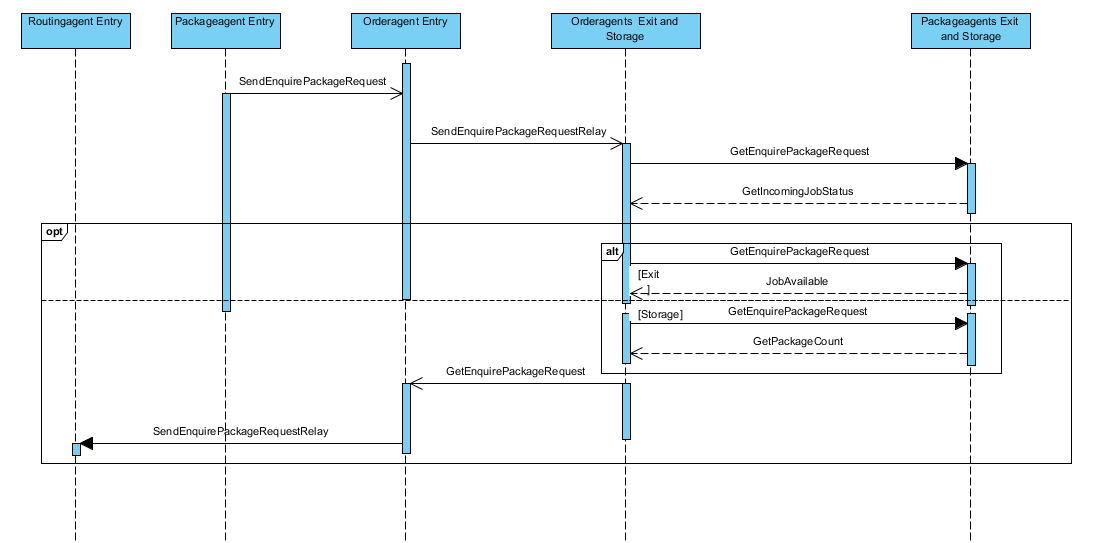
\includegraphics[width=1.1\textwidth, height=0.6\textwidth]{EingangAusgang.png}        
		\caption{Eingang fragt Ausgang und Zwischenlager}
	\label{Eingang fragt}
\end{figure}
\paragraph{Ausgang fragt Zwischenlager}
Pakete, die am Eingang eintreffen und für die noch keine Nachfrage an den Ausgangsrampen besteht, werden ins Zwischenlager gebracht. Damit auch diese Pakete zum Ausgang gelangen, fragt der Ausgang zyklisch im Zwischenlager für die entsprechenden Pakete nach. Abbildung \ref{Ausgang fragt} zeigt den Ablauf im Detail:
\begin{itemize}
\item Der Paketagent des Ausgangs stellt mithilfe einer Tickerbehaviour zyklisch Anfragen an seinen Orderagenten, damit im Zwischenlager geprüft wird, ob ein Paket vorhanden ist, für das eine Nachfrage besteht. Bevor der Orderagent benachrichtigt wird, prüft der Paketagent mithilfe der Variable IncomingJobFlag, ob bereits ein Paket erwartet wird. Falls nicht, sendet er die Anfrage an den Orderagenten.  
\item Der Orderagent sendet eine Nachricht an alle Orderagenten der Zwischenrampen.
\item Der jeweilige Orderagent fragt seinen Paketagenten, ob bereits ein Paket abgeholt wird. Dies ist nötig, damit sich nicht mehrere Bots vor einer Rampe blockieren und damit ein Bot nicht das falsche Paket abholt.
\item Der Paketagent prüft anhand der Variable OutgoingJobFlag, ob ein Paket erwartet wird und antwortet seinem Orderagenten.
\item Sofern kein Paket erwartet wird, fährt der Orderagent fort und stellt eine erneute Anfrage an seinen Paketagenten, um zu fragen, ob das Paket, das der Ausgang verlangt, an vorderster Stelle der Rampe ist.
\item Der jeweilige Orderagent antwortet dem Ausgang, ob das Paket vorhanden ist oder nicht.
\item Sofern das Paket in einem der Zwischenlager ist, benachrichtigt der Orderagent des Ausgangs den Routingagenten des Zwischenlagers, damit das Paket von einem Bot abgeholt wird. 
\end{itemize} 
\begin{figure}[h!]
	\centering
		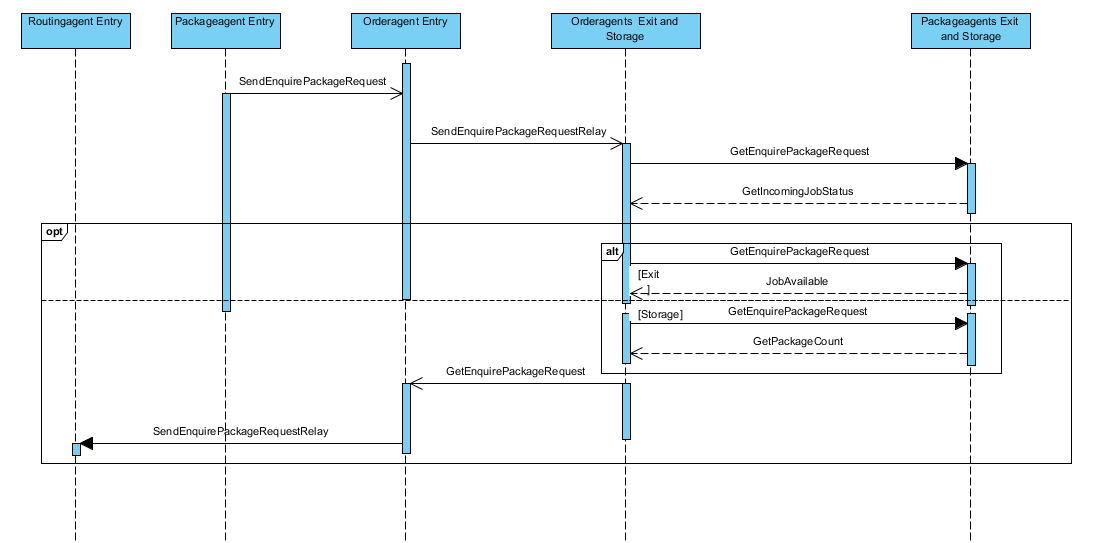
\includegraphics[width=1.1\textwidth, height=0.6\textwidth]{EingangAusgang.png}        
		\caption{Ausgang fragt Zwischenlager}
	\label{Ausgang fragt}
\end{figure}
\paragraph{Auktion}
Nachdem ein Paket ein Ziel zugewiesen bekommen hat, startet der Routingagent der jeweiligen Eingangs- oder Zwischenrampe eine Auktion, um ein Fahrzeug zu finden, das das Paket befördert. Abbildung \ref{Auktion} zeigt den Ablauf der Auktion:
\begin{itemize}
\item Der Routingagent schickt eine Nachricht an alle Routingagenten der Fahrzeuge.
\item Die Routingagenten der Fahrzeuge fragen ihre Paketagenten, ob bereits ein Auftrag durchgeführt wird. Der Routingagent wartet bis der Paketagent geantwortet hat.
\item Der Paketagent antwortet dem Routingagenten.
\item Falls das Fahrzeug nicht belegt ist und der Bot auch an keiner anderen Auktion teilnimmt, erfragt der Routingagent seine aktuelle Position von seinem Plattformagenten.
\item Der Plattformagent schickt die aktuelle Position an den Routingagenten.
\item Der Routingagent berechnet mithilfe des Pathfindings eine Aufwandsabschätzung und schickt Sie dem Routingagenten der Rampe. Falls er nicht in der Lage ist, ein Paket zu befördern, teilt er dies der Rampe über die Nachricht mit.
\item Der Routingagent der Rampe speichert alle Estimations nacheinander ab. Haben alle Fahrzeuge geantwortet oder ist der Timeout für die Auktion abgelaufen, wird, sofern vorhanden, der Bot mit der besten Estimation ausgewählt. Falls es einen Bot gibt, der das Paket abholen kann, wird der Paketagent des Zwischenlagers oder Ausgangs benachrichtigt, dass ein Paket in Kürze geliefert wird, damit das IncomingJobFlag gesetzt wird. Dadurch wird verhindert, dass die Bots sich gegenseitig vor einer Rampe blockieren.
\item Der Paketagent antwortet dem Routingagenten nach dem Setzen des Flags.
\item Der Routingagent teilt dem Routingagenten des ausgewählten Fahrzeugs mit, dass es ausgewählt wurde.
\item Der Routinagent des Fahrzeugs sendet eine Nachricht an seinen Paketagenten, um Platz für das Paket zu reservieren.
\item Der Fahrzeug Routingagent leitet die Information an seinen Plattformagenten weiter, damit die Fahrt beginnen kann.
\end{itemize}
\begin{figure}[h!]
	\centering
		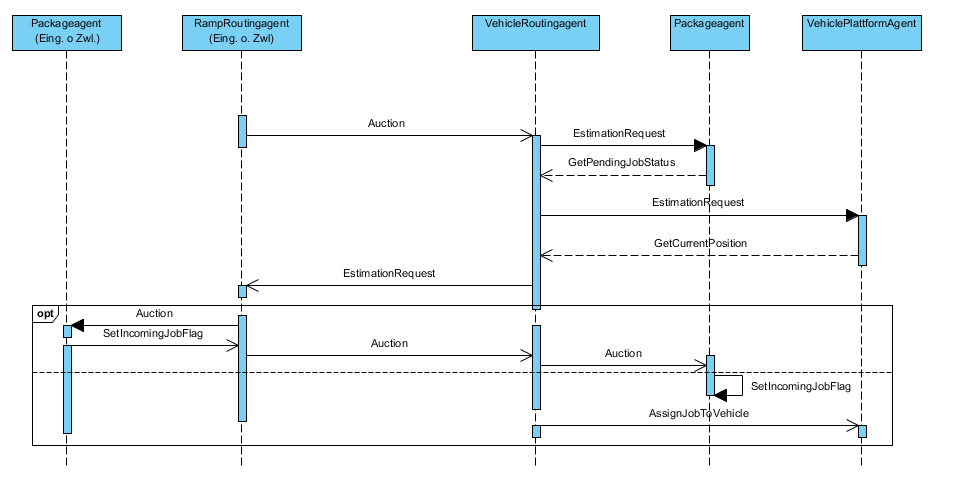
\includegraphics[width=1.1\textwidth, height=0.6\textwidth]{Auktion.PNG}        
		\caption{Auktion}
	\label{Auktion}
\end{figure}
\paragraph{Paket von Startrampe abholen und zur Zielrampe bringen}
Nachdem das Fahren initiiert wurde, führt der Plattformagent des entsprechenden Fahrzeugs den Transport durch. Abbildung \ref{Fahren} zeigt den Ablauf auf Agentenebene:
\begin{itemize}
\item Das Fahrzeug fährt zur Startrampe und benachrichtigt den Plattformagenten der jeweiligen Rampe.
\item Dieser benachrichtigt seinen Paketagenten, dass das Paket transferiert werden kann. 
\item Der Paketagent sendet eine Nachricht an den Paketagenten des Fahrzeugs, um das Paket zu übergeben und entfernt es von der Rampe.
\item Der Paketagent des Fahrzeugs fügt das Paket hinzu und antwortet dem anderen Paketagenten.
\item Der Paketagent der Startrampe  benachrichtigt den Plattformagenten, dass das Paket übergeben wurde.
\item Dieser benachrichtigt wiederum den Plattformagenten des Fahrzeugs, damit dieser weiß, dass er weiterfahren kann.
\item Der Plattformagent des Fahrzeugs fährt zur Zielrampe und benachrichtigt seinen Paketagenten, dass das Paket übergeben werden kann.
\item Der Paketagent entfernt das Paket und sendet eine Nachricht an den Paketagenten der Rampe, dass das Paket aufgenommen werden soll.
\item Dieser fügt das Paket hinzu und gibt dem Paketagent des Fahrzeugs Bescheid, dass das Aufladen beendet ist.
\item Der Fahrzeug Paketagent informiert seinen Plattformagent, dass der Auftrag erledigt ist.
\end{itemize}
\begin{figure}[h!]
	\centering
		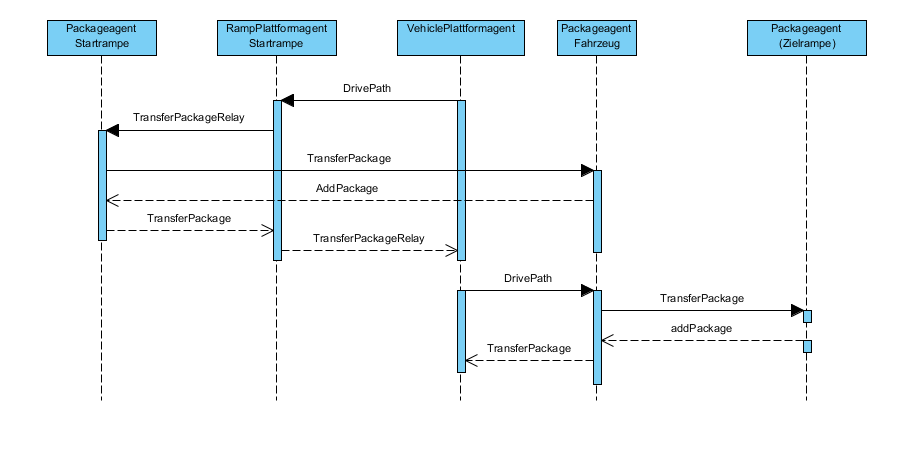
\includegraphics[width=1.1\textwidth, height=0.6\textwidth]{Fahren.PNG}        
		\caption{Paket abholen und zur Zielrampe bringen}
	\label{Fahren}
\end{figure}
\subsubsection{Implementierung des Pathfindings}
% TODO
\subsubsection{Implementierung der Statistiken}
% TODO
\subsubsection{Interaktion der Komponenten}
In Abschnitt \ref{Interaktion der Komponenten} wurden die Interaktionen der Systemkomponenten auf logischer Ebene beschrieben, die für das Starten einer Simulation bis hin zur Visualisierung notwendig sind. Im Folgenden Abschnitt soll beschrieben werden, wie und mit welchen Mitteln die einzelnen Schritte implementiert wurden. 
\paragraph{Client-Server Kommunikation}
Das Starten einer Simulation wird über das Menuitem \glqq Starten/Anhalten\grqq ausgelöst (s. Abbildung\ref{RPCS}). Wird das Menuitem gedrückt, dann wird die Methode execute ausgeführt. In der Methode wird geprüft, ob die Simulation bereits läuft, um festzustellen, ob die Simulation gestartet oder angehalten werden soll. Wenn die Simulation noch nicht gestartet wurde, wird zunächst geprüft, ob das erstellte Szenario konsistent ist (Mindestens eine Eingangs- und Ausgangsrampe). Wenn dies der Fall ist, wird die Simulation gestartet. Dies erfordert eine Client-Server Kommunikation. Die Implementierung erfolgt durch den von GWT bereitgestellten Remote Procedure Call (RPC) Mechanismus (Vgl. \cite{gwtrpc}). 
\\\\
Die  Variable agentPlatformService referenziert das Interface AgentPlatformServiceAsync. Serverseitig gibt es ein Servlet \glqq AgentPlatformService\grqq , das verschiedene Methoden bereitstellt, die über das Interface AgentPlatformServiceAsync aufgerufen werden können. Die Variable ist als AgentPlatformServiceAsync Interface deklariert, wird aber mit einer automatisch generierten Proxy-Klasse instantiiert (s. Quellcode/Konstruktor der Klasse MainframePresenter). In der Methode execute wird über den Aufruf der Methode startSimulation das Szenario übergeben und zum Server geschickt. Für den Aufruf ist ein Objekt notwendig, das das Interface AsyncCalback implementiert, welches wiederum der Methode als interne Klasse übergeben wird. Der Typparameter, in diesem Fall ein Integer, definiert, welcher Rückgabewert vom Server erwartet wird. Außerdem wird in den Methoden onFailure und onSuccess definiert, was passieren soll, wenn der RPC fehlschlägt bzw. erfolgreich war. Wenn die Simulation serverseitig erfolgreich gestartet wurde, dann soll die auf dem Server generierte ID dem aktuellen Szenario zugewiesen werden und der Status der Simulation auf gestartet gesetzt werden.    
\begin{figure}[h!]
	\centering
		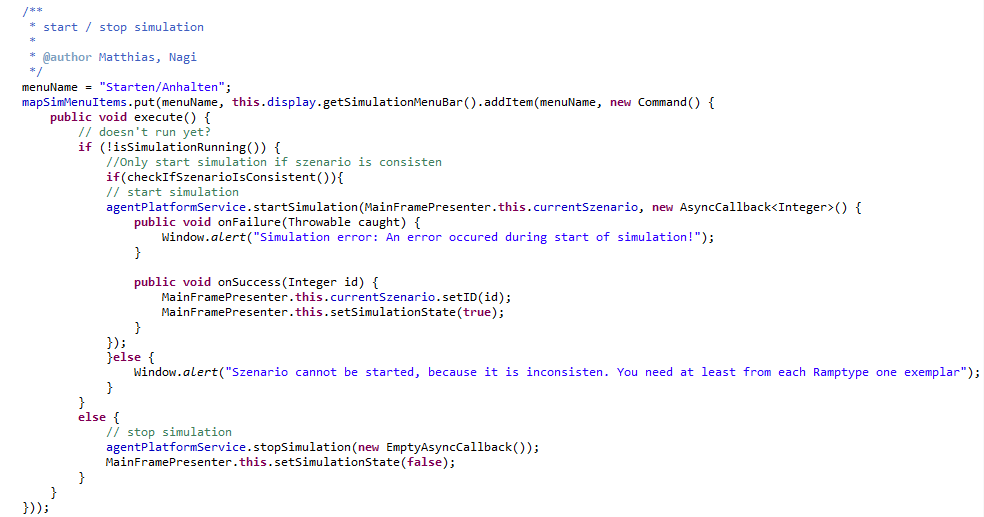
\includegraphics[width=1.1\textwidth, height=0.6\textwidth]{RPCS.PNG}        
		\caption{Starten einer Simulation}
	\label{RPCS}
\end{figure}
\paragraph{Start des Multiagenten-Systems}
Nachdem die Daten zum Server geschickt wurden, wird die Methode startSimulation des Servlets AgentPlatformServiceImpl aufgerufen. Für das Szenario wird eine ID generiert und über das Object Array wird das Szenario allen Agenten als Parameter zur Verfügung gestellt. Danach wird eine Agentenplattform für das jeweilige Szenario gestartet. Die Liste der Conveyor aus dem Szenario wird durchlaufen und für jeden Conveyor werden die benötigten Agenten erzeugt. Die Methode addAgentToSimulation erzeugt anhand der Conveyor- und Szenario-ID einen eindeutigen Namen für jeden Agenten, übergibt die Parameter und fügt ihn der Simulation hinzu. Anschließend wird der Jobagent initialisiert und die Agenten werden gestartet. Die letzte Anweisung schickt die Szenario ID zum Client zurück.  
\begin{figure}[h!]
	\centering
		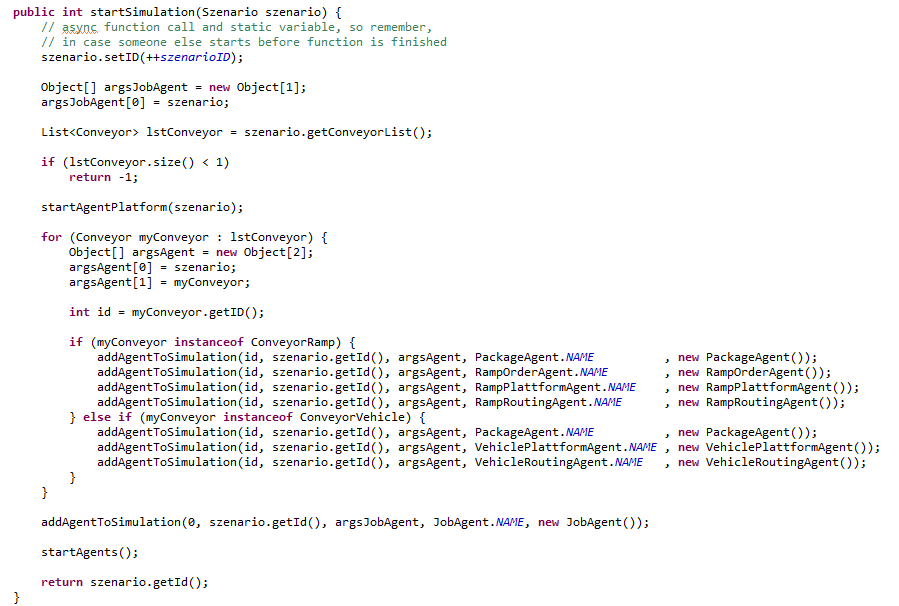
\includegraphics[width=1.1\textwidth, height=0.6\textwidth]{StartMAS.PNG}        
		\caption{Starten des MAS}
	\label{SMAS}
\end{figure}
\paragraph{Start des Jobtimers} 
Nachdem der Jobagent alle Informationen erhalten hat, die er für die Zuweisung von Aufträgen benötigt, schickt er eine Nachricht an den Client, dass die Aufträge zum Server geschickt werden können (Vgl.Abschnitt \ref{Jobagent}). Der Client startet den Jobtimer mit der Methode startJobTimer des MainframePresenters (s.Abbildung \ref{jobtim}). Die Integer Variable elapsedTimeSec repräsentiert die Zeit. Der Timer wird gestartet und die run-Methode wird kontinuierlich ausgeführt, bis der Jobtimer gestoppt wird. Die Zeitvariable wird bei jedem Durchlauf um eins hochgezählt, was bedeutet, dass eine Sekunde vergangen ist. Die einzelnen Jobs aus der Liste werden in der for-Schleife abgefragt und ihr Zeitstempel wird mit der elapsedTimeSec Variable abgeglichen. Ist die vergangene Zeit größer oder gleich der Zeit zu der ein Job ausgeführt werden soll, dann wird der Job mit der Methode addJob zum Server geschickt. Mit der vorletzten Anweisung wird festgelegt, in welchen Zeitabständen der Timer ausgeführt werden soll. Die letzte Anweisung dient dazu, den Timer initial zu starten.
\begin{figure}[h!]
	\centering
		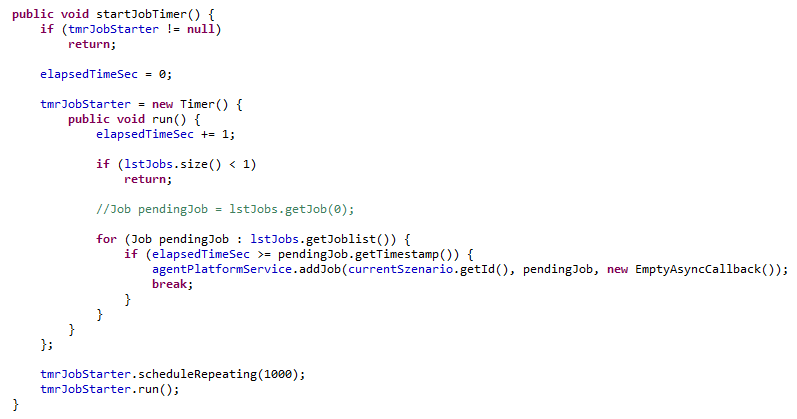
\includegraphics[width=1.1\textwidth, height=0.6\textwidth]{Jobtimer.PNG}        
		\caption{Start des Jobtimers}
	\label{jobtim}
\end{figure}
\\\\
Abbildung \ref{jobtimserv} zeigt die serverseitige Weiterleitung des empfangenen Auftrags. In der Methode addJob des AgentPlatformServiceImpl Servlets wird der jeweilige Jobagent anhand der Szenario ID aus einer Hashmap geholt. Es wird ein ACLMessageObjekt erzeugt und der Nachrichtentyp wird im Konstruktor festgelegt, um gezielt die notwendige Behaviour zu adressieren. Als Empfänger wird der Jobagent selber festgelegt. Anschließend wird der Job der Nachricht als ContentObject hinzugefügt und versendet.
\begin{figure}[h!]
	\centering
		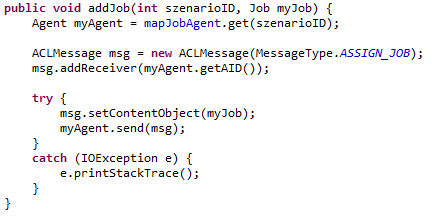
\includegraphics[width=1.1\textwidth, height=0.6\textwidth]{addJob.PNG}        
		\caption{Weiterleitung des Auftrags}
	\label{jobtimserv}
\end{figure}
\paragraph{Visualisierung von Zustandsveränderungen}
Die einzelnen Agenten führen Aktionen durch. Werden dadurch Zustände verändert (z.~B. Hinzufügen eines Pakets etc.), müssen diese visualisiert werden. Das MAS läuft auf dem Server. Damit ein Client die Zustandsveränderungen visualisieren kann, muss er vom Server über die Art der Zustandsveränderung informiert werden. Das Schicken von Nachrichten vom Server zum Client wurde mithilfe des GWT Eventservices implementiert. Der Eventservice ist ein event-basiertes Kommunikationsframework, dass auf dem GWT-RPC Mechanismus und der Comet Server-Push Technologie basiert (Vgl. \cite{gwteventservice}). Abbildung \ref{addEvent} zeigt die Methode AddPackage des Packageagents, die für das Hinzufügen eines Pakets benötigt wird. Nachdem das Paket in die Liste eingefügt wurde, wird mithilfe der Klasse EventHelper ein Event zum Client gefeuert. Der EventHelper erbt von dem Servlet RemoteEventServiceServlet, das vom EventService Framework bereitgestellt wird und das GWT-Servlet, um die Funktionalität zum Versenden von Events erweitert (Vgl.\cite{gwteventservice}). 
\\\\
Die Klasse PackageAddedEvent ist eine selbst definierte Event-Klasse, die das Interface Event des Eventservices implementiert (Vgl.\cite{gwteventservice}). Mithilfe dieser Klasse können Informationen für den Client transportiert werden. Die Informationen werden im Konstruktor der Klasse PackageAddedEvent übergeben. In diesem Fall werden die Conveyor- und Package-ID übergeben, damit der Client weiß, welchen Conveyor er neu zeichnen soll und welches Paket mit welcher ID hinzugefügt wurde.
\begin{figure}[h!]
	\centering
		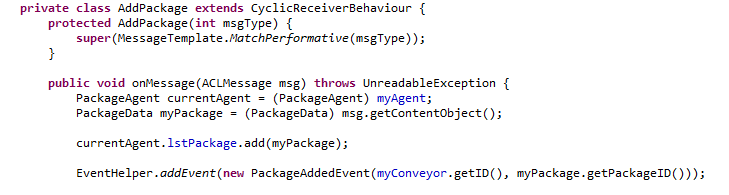
\includegraphics[width=1.1\textwidth, height=0.6\textwidth]{addEvent.PNG}        
		\caption{Feuern eines Events}
	\label{addEvent}
\end{figure}
\\\\
Abbildung \ref{addEventClient} zeigt die clientseitige Verarbeitung der Events, die vom Server empfangen werden. In der Methode HandleEvents des Mainframepresenters , wird zunächst eine Instanz der Klasse RemoteEventService über die RemoteEventServiceFactory geliefert. Alle vorhandenen Listener werden entfernt und es wird ein neuer Listener hinzugefügt. Beim Hinzufügen des Listeners wird eine Domain mit einer Zeichenkette übergeben. Durch die Domain kann gezielt festgelegt werden, für wen eine Nachricht bestimmt ist (Vgl.\cite{gwteventservice}). Die Zuordnung einer Nachricht zu einer Domain, wird beim Versenden der Nachricht festgelegt (S. Quellcode Klasse EventHelper). In der Methode apply des Listeners wird für alle definierten Events festgelegt, welche Aktion beim Empfang auf dem Client ausgeführt werden soll. Beispielsweise wird durch das SimStartedEvent das Starten des Jobtimers durch die Methode startJobTimer initialisiert.  
\begin{figure}[h!]
	\centering
		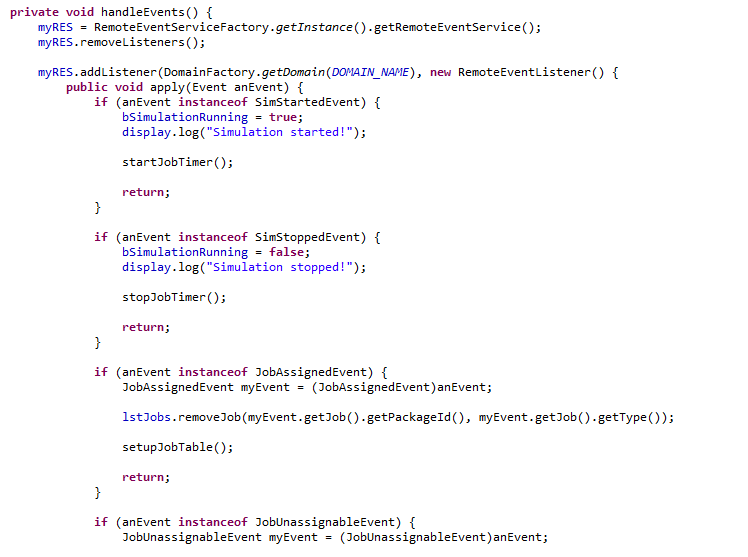
\includegraphics[width=1.1\textwidth, height=0.6\textwidth]{Vis.PNG}        
		\caption{Clientseitige Verarbeitung des Events}
	\label{addEventClient}
\end{figure} 
